\documentclass{article} % For LaTeX2e
\usepackage{nips15submit_e,times}
\usepackage{hyperref}
\usepackage{url}
\usepackage{graphicx}
\graphicspath{ {/Users/Tyler/LOVEFest/Figures/pdf/} }
%\documentstyle[nips14submit_09,times,art10]{article} % For LaTeX 2.09


\title{Randomer Forests}


\author{
Tyler M. Tomita\thanks{ Use footnote for providing further information
about author (webpage, alternative address)---\emph{not} for acknowledging
funding agencies.} \\
Department of Biomedical Engineering\\
Johns Hopkins University\\
Baltimore, MD \\
\texttt{ttomita@jhu.edu} \\
\And
Joshua T. Vogelstein \\
Department of Biomedical Engineering \\
Johns Hopkins University \\
\texttt{email} \\
\AND
Coauthor \\
Affiliation \\
Address \\
\texttt{email} \\
\And
Coauthor \\
Affiliation \\
Address \\
\texttt{email} \\
\And
Coauthor \\
Affiliation \\
Address \\
\texttt{email} \\
(if needed)\\
}

% The \author macro works with any number of authors. There are two commands
% used to separate the names and addresses of multiple authors: \And and \AND.
%
% Using \And between authors leaves it to \LaTeX{} to determine where to break
% the lines. Using \AND forces a linebreak at that point. So, if \LaTeX{}
% puts 3 of 4 authors names on the first line, and the last on the second
% line, try using \AND instead of \And before the third author name.

\newcommand{\fix}{\marginpar{FIX}}
\newcommand{\new}{\marginpar{NEW}}

%\nipsfinalcopy % Uncomment for camera-ready version

\begin{document}

\maketitle

\begin{abstract}
Insert abstract
\end{abstract}

\section{Introduction}
Insert introduction

\section{Methods}
Insert methods

\section{Results}
Talk about figures

\section{Discussion}
Insert discussion

\begin{figure}[h]
\begin{center}
%\framebox[4.0in]{$\;$}
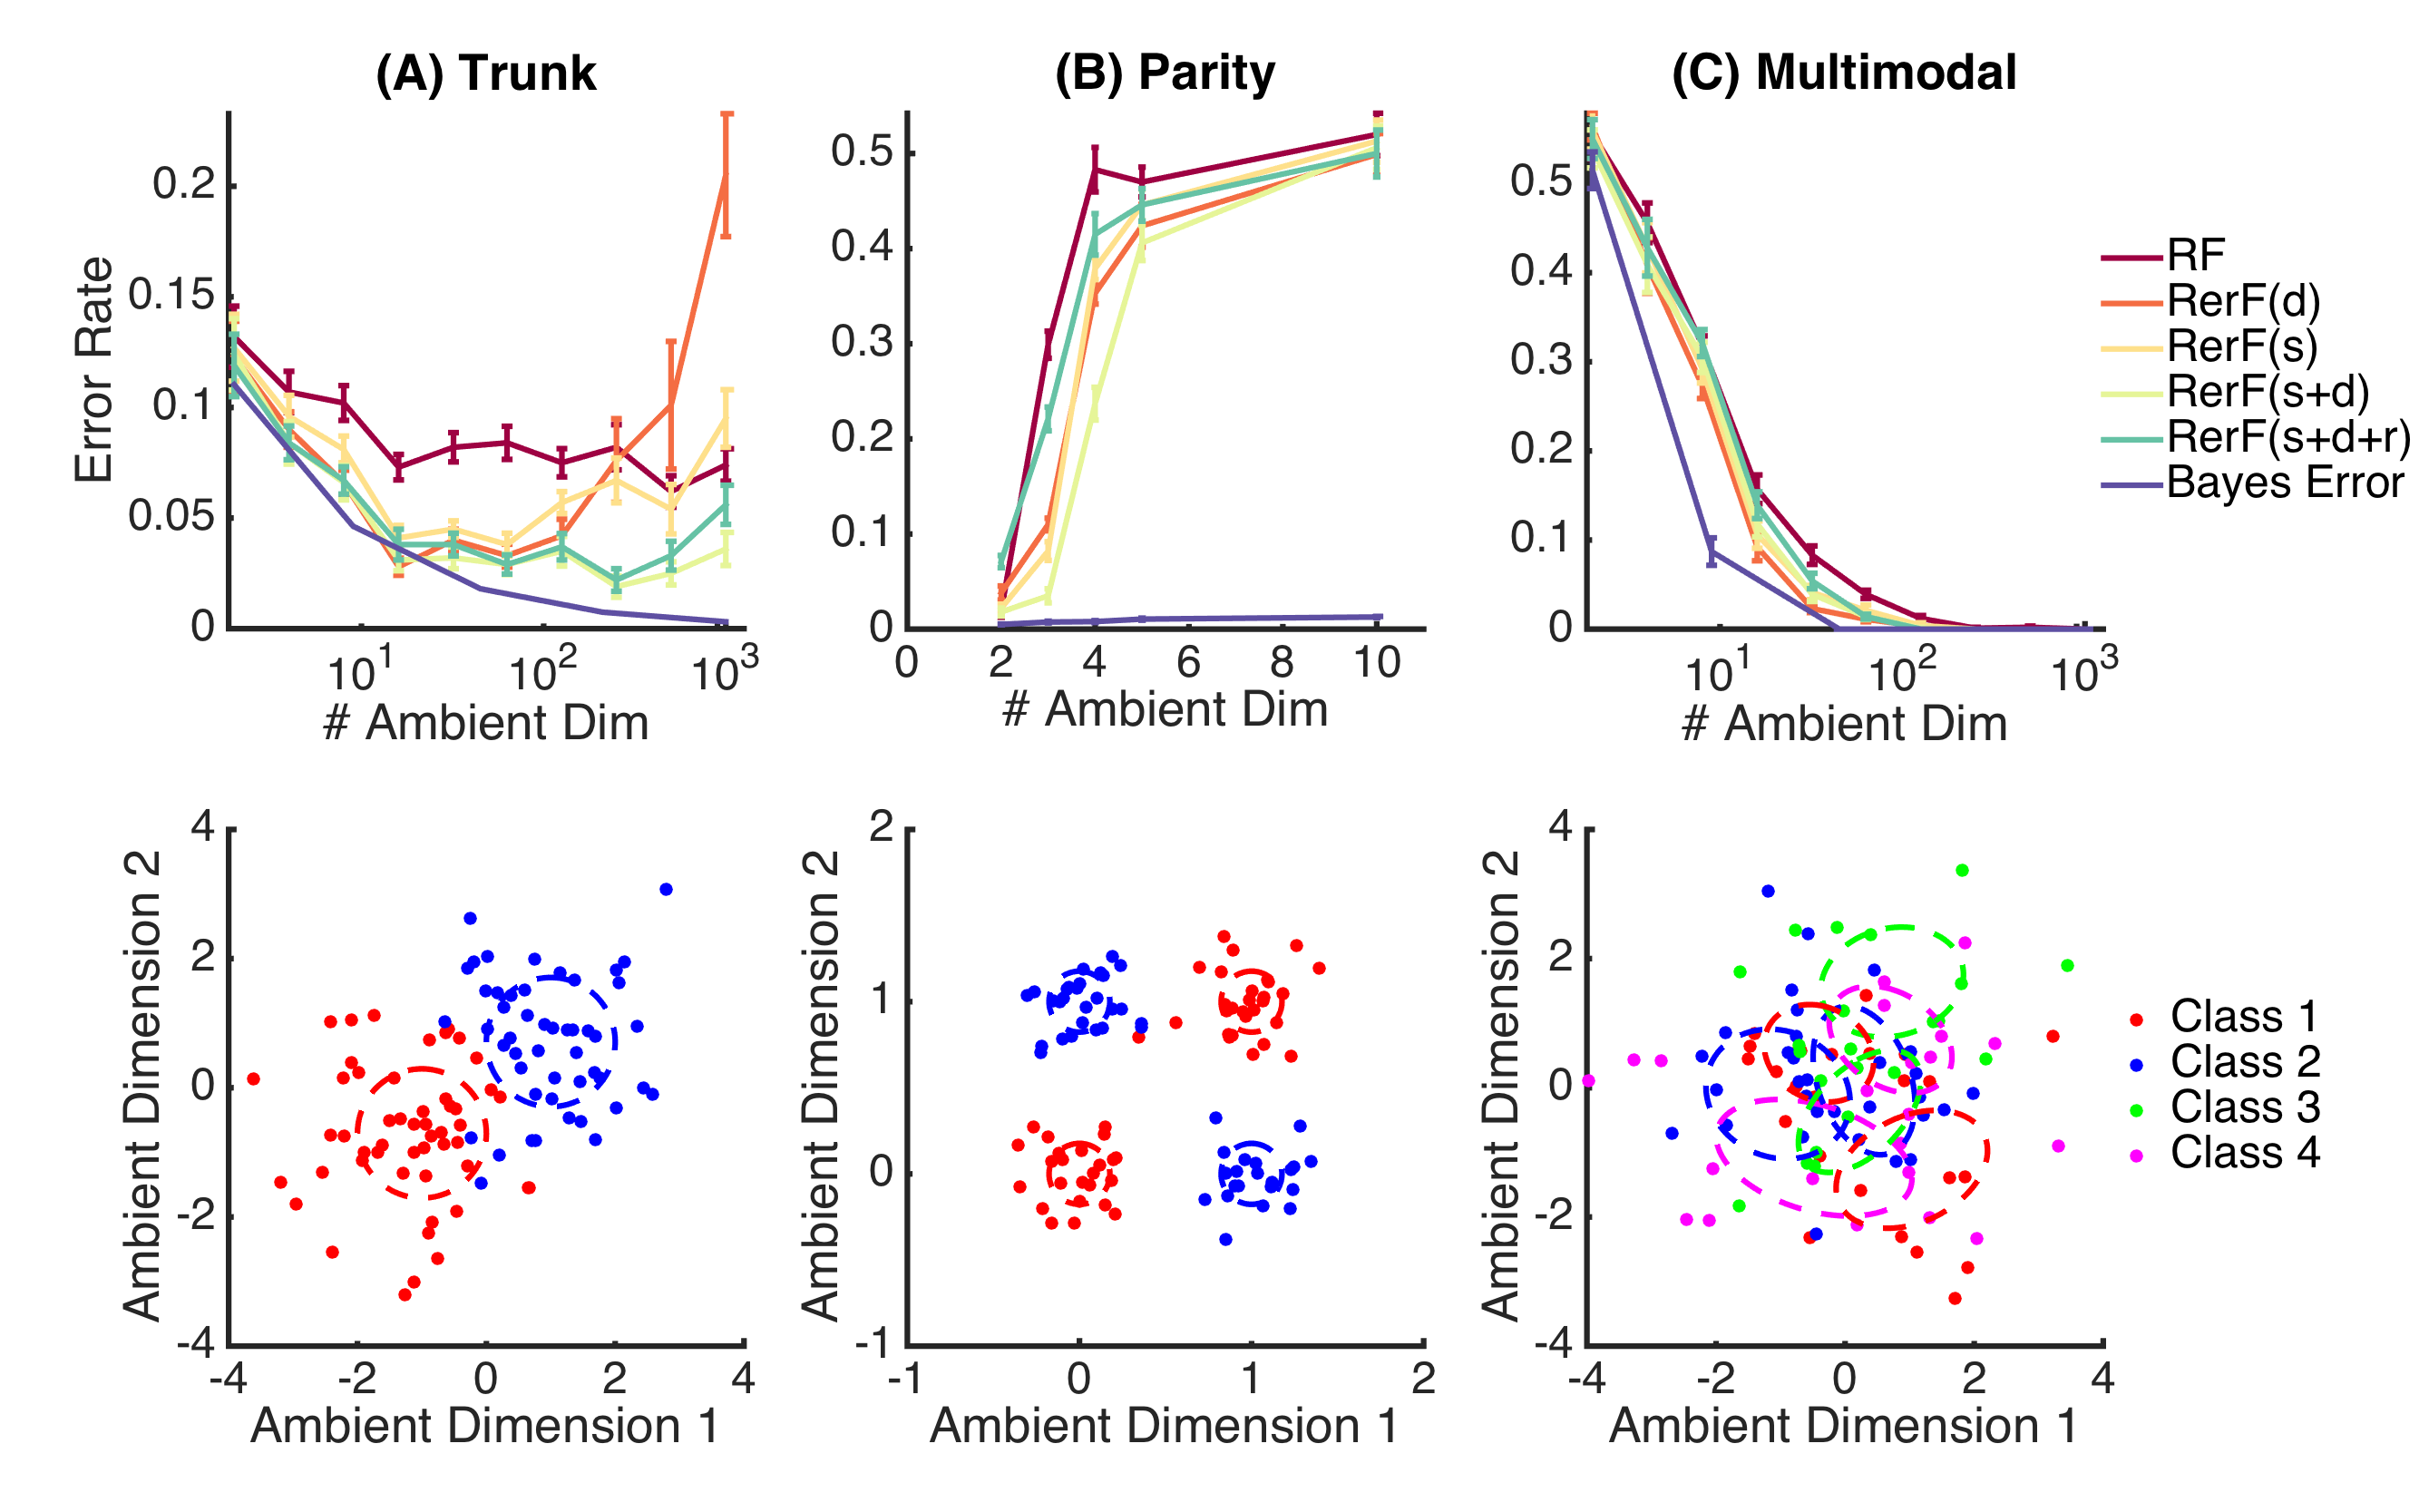
\includegraphics[trim=0in 0.4in 0in 0.4in, clip=true, width=\linewidth]{Fig1_Lhat}
\end{center}
\caption{Classification performance comparing Random Forest (RF) to several variants of Randomer Forest (R'er F), and Bayes optimal performance, on three distinct simulation settings: (A) Trunk, (B) Parity, and (C) Multimodal (see Methods for details).  For all settings, the top panel depicts misclassification rate vs. the number of ambient (coordinate) dimensions, and the bottom panel shows a 2D scatter plot of the first 2 coordinates (dashed circles denote the standard deviation level set).  Note that in all settings, for all number of dimensions, R'er F outperforms RF, even Trunk and Parity, which were designed specifically for RF because the discriminant boundary naturally lies along the coordinate basis.}
\end{figure}

\begin{figure}[h]
\begin{center}
%\framebox[4.0in]{$\;$}
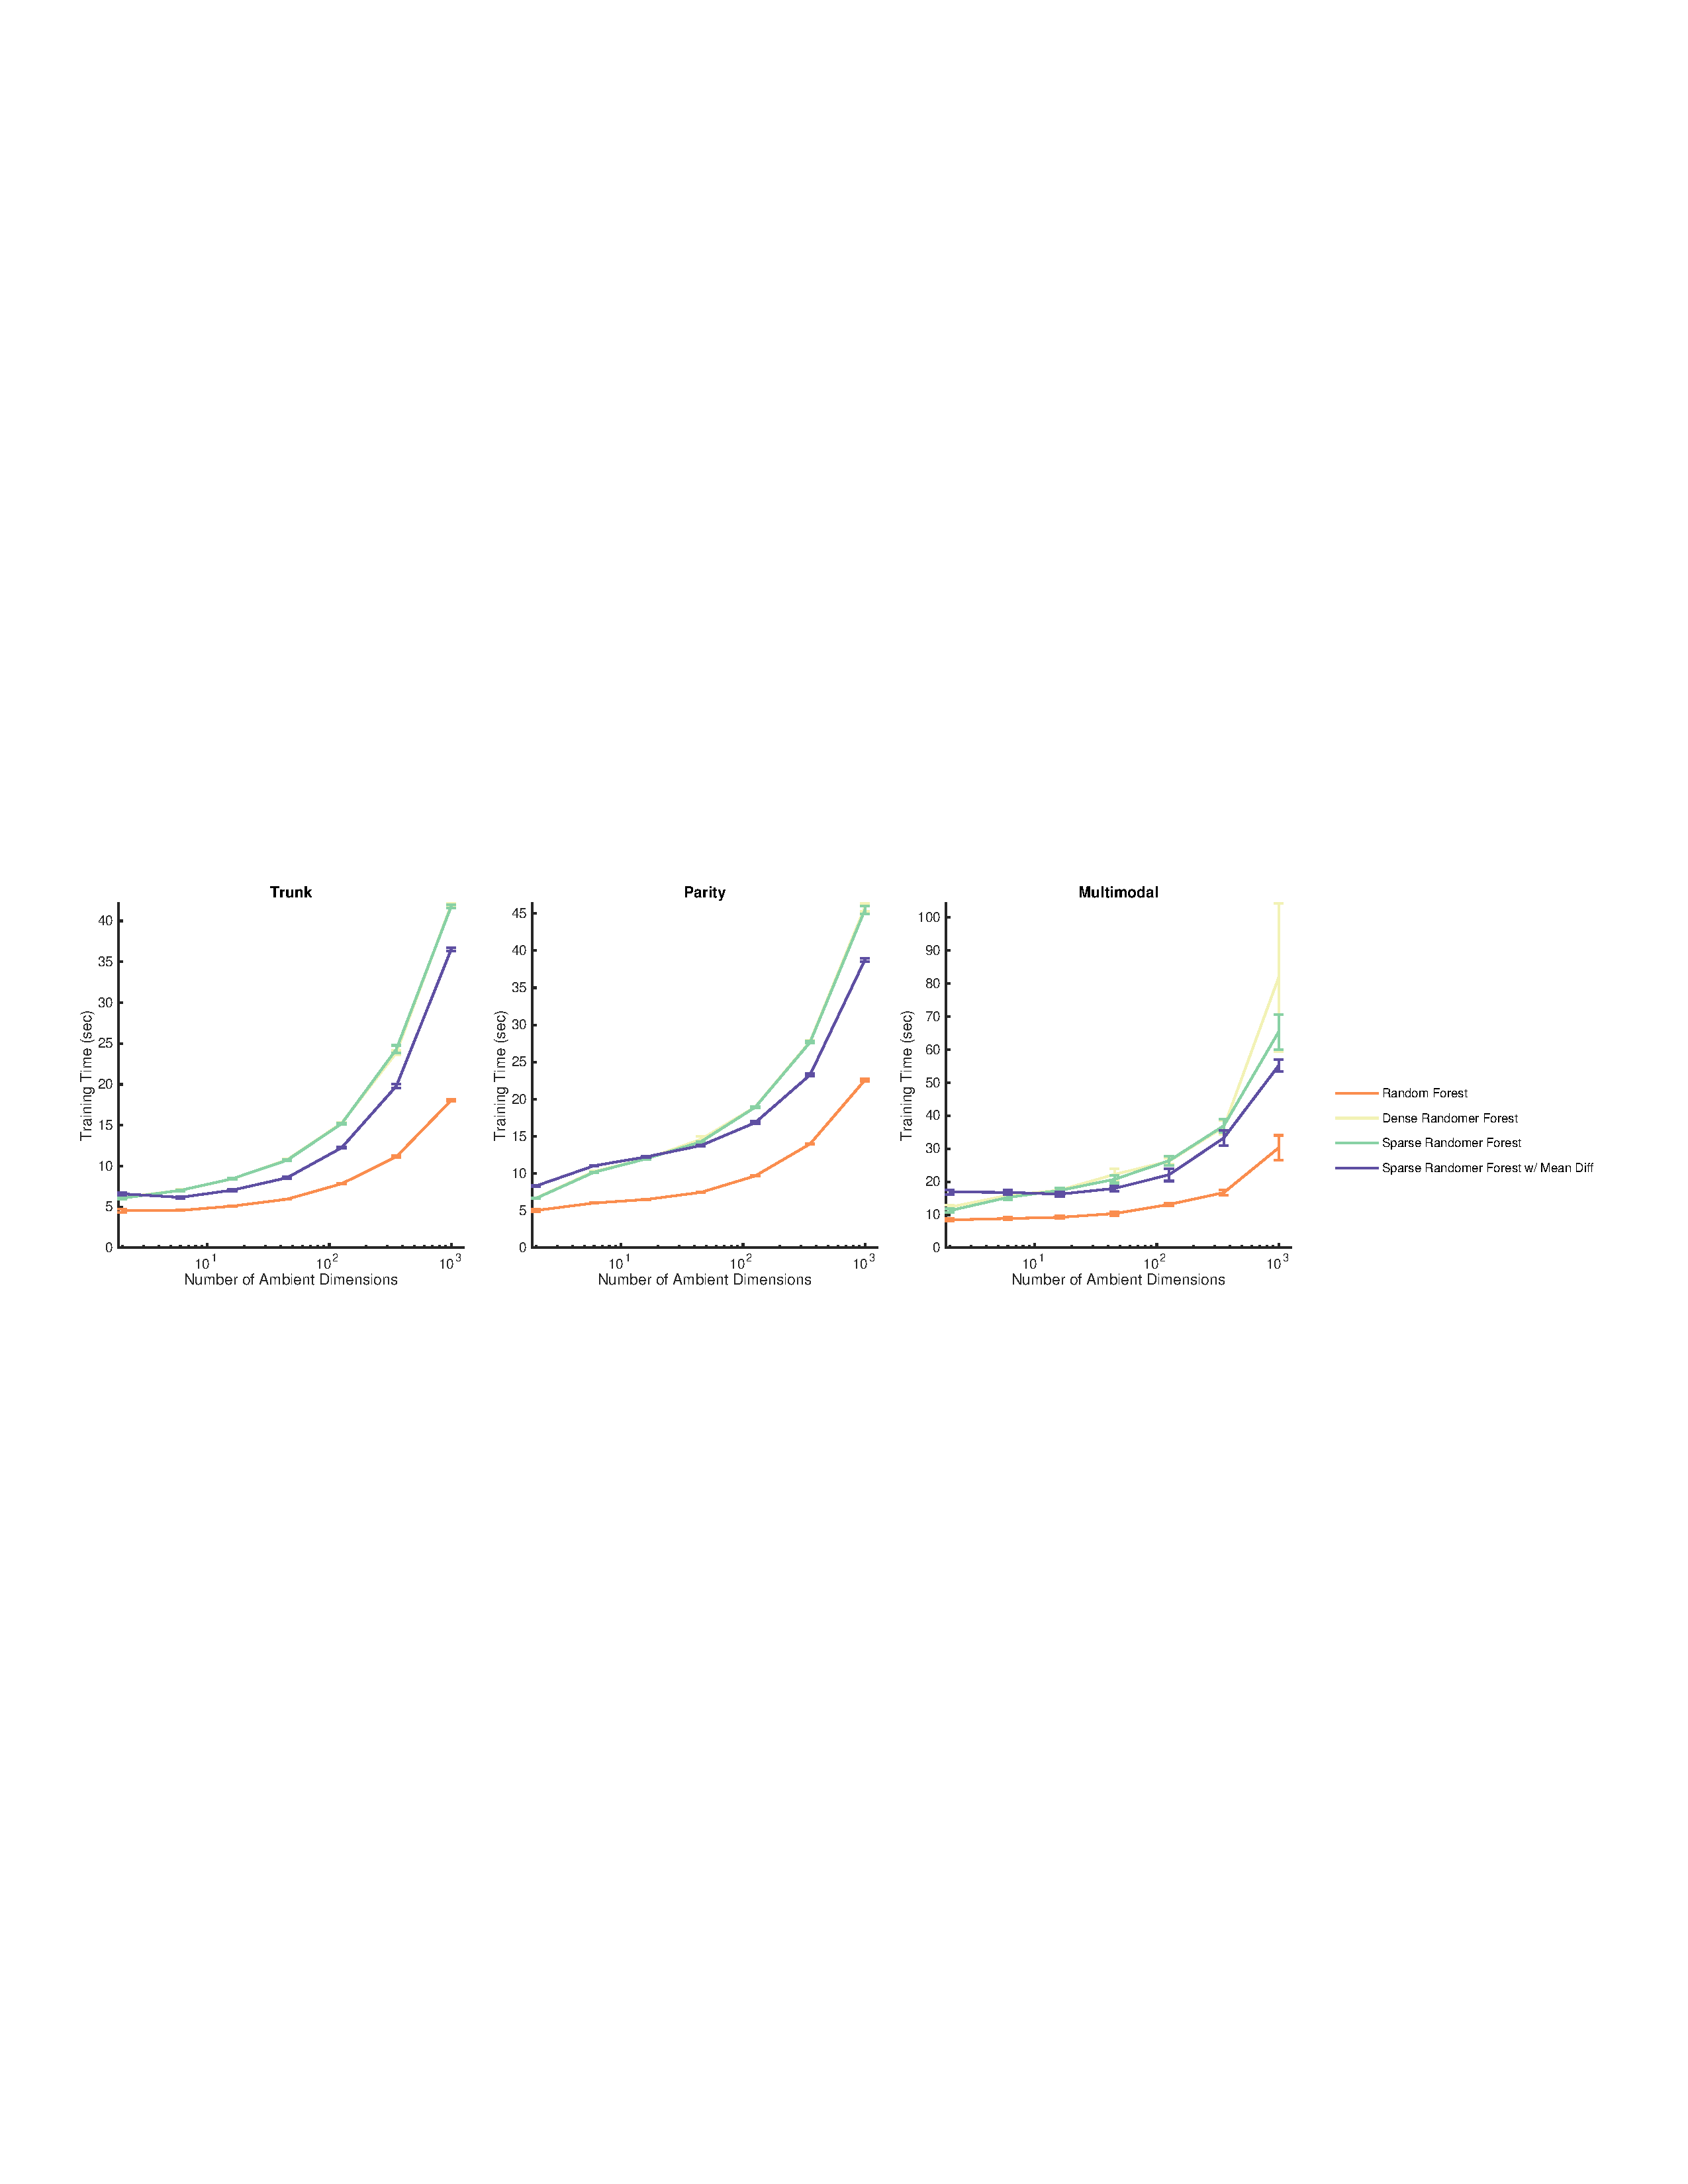
\includegraphics[trim=0in 3in 0in 3in, clip=true, width=\linewidth]{Fig2_Time}
\end{center}
\caption{Classifier training time comparing RF to several variants of R'er F, same setting as the top row of Figure 1. The only difference is that the y-axis here labels training time (in seconds). Although R'er F requires slightly more time than RF (largely due to random sampling of projection matrices), they scale similarly.}
\end{figure}

\begin{figure}[h]
\begin{center}
%\framebox[4.0in]{$\;$}
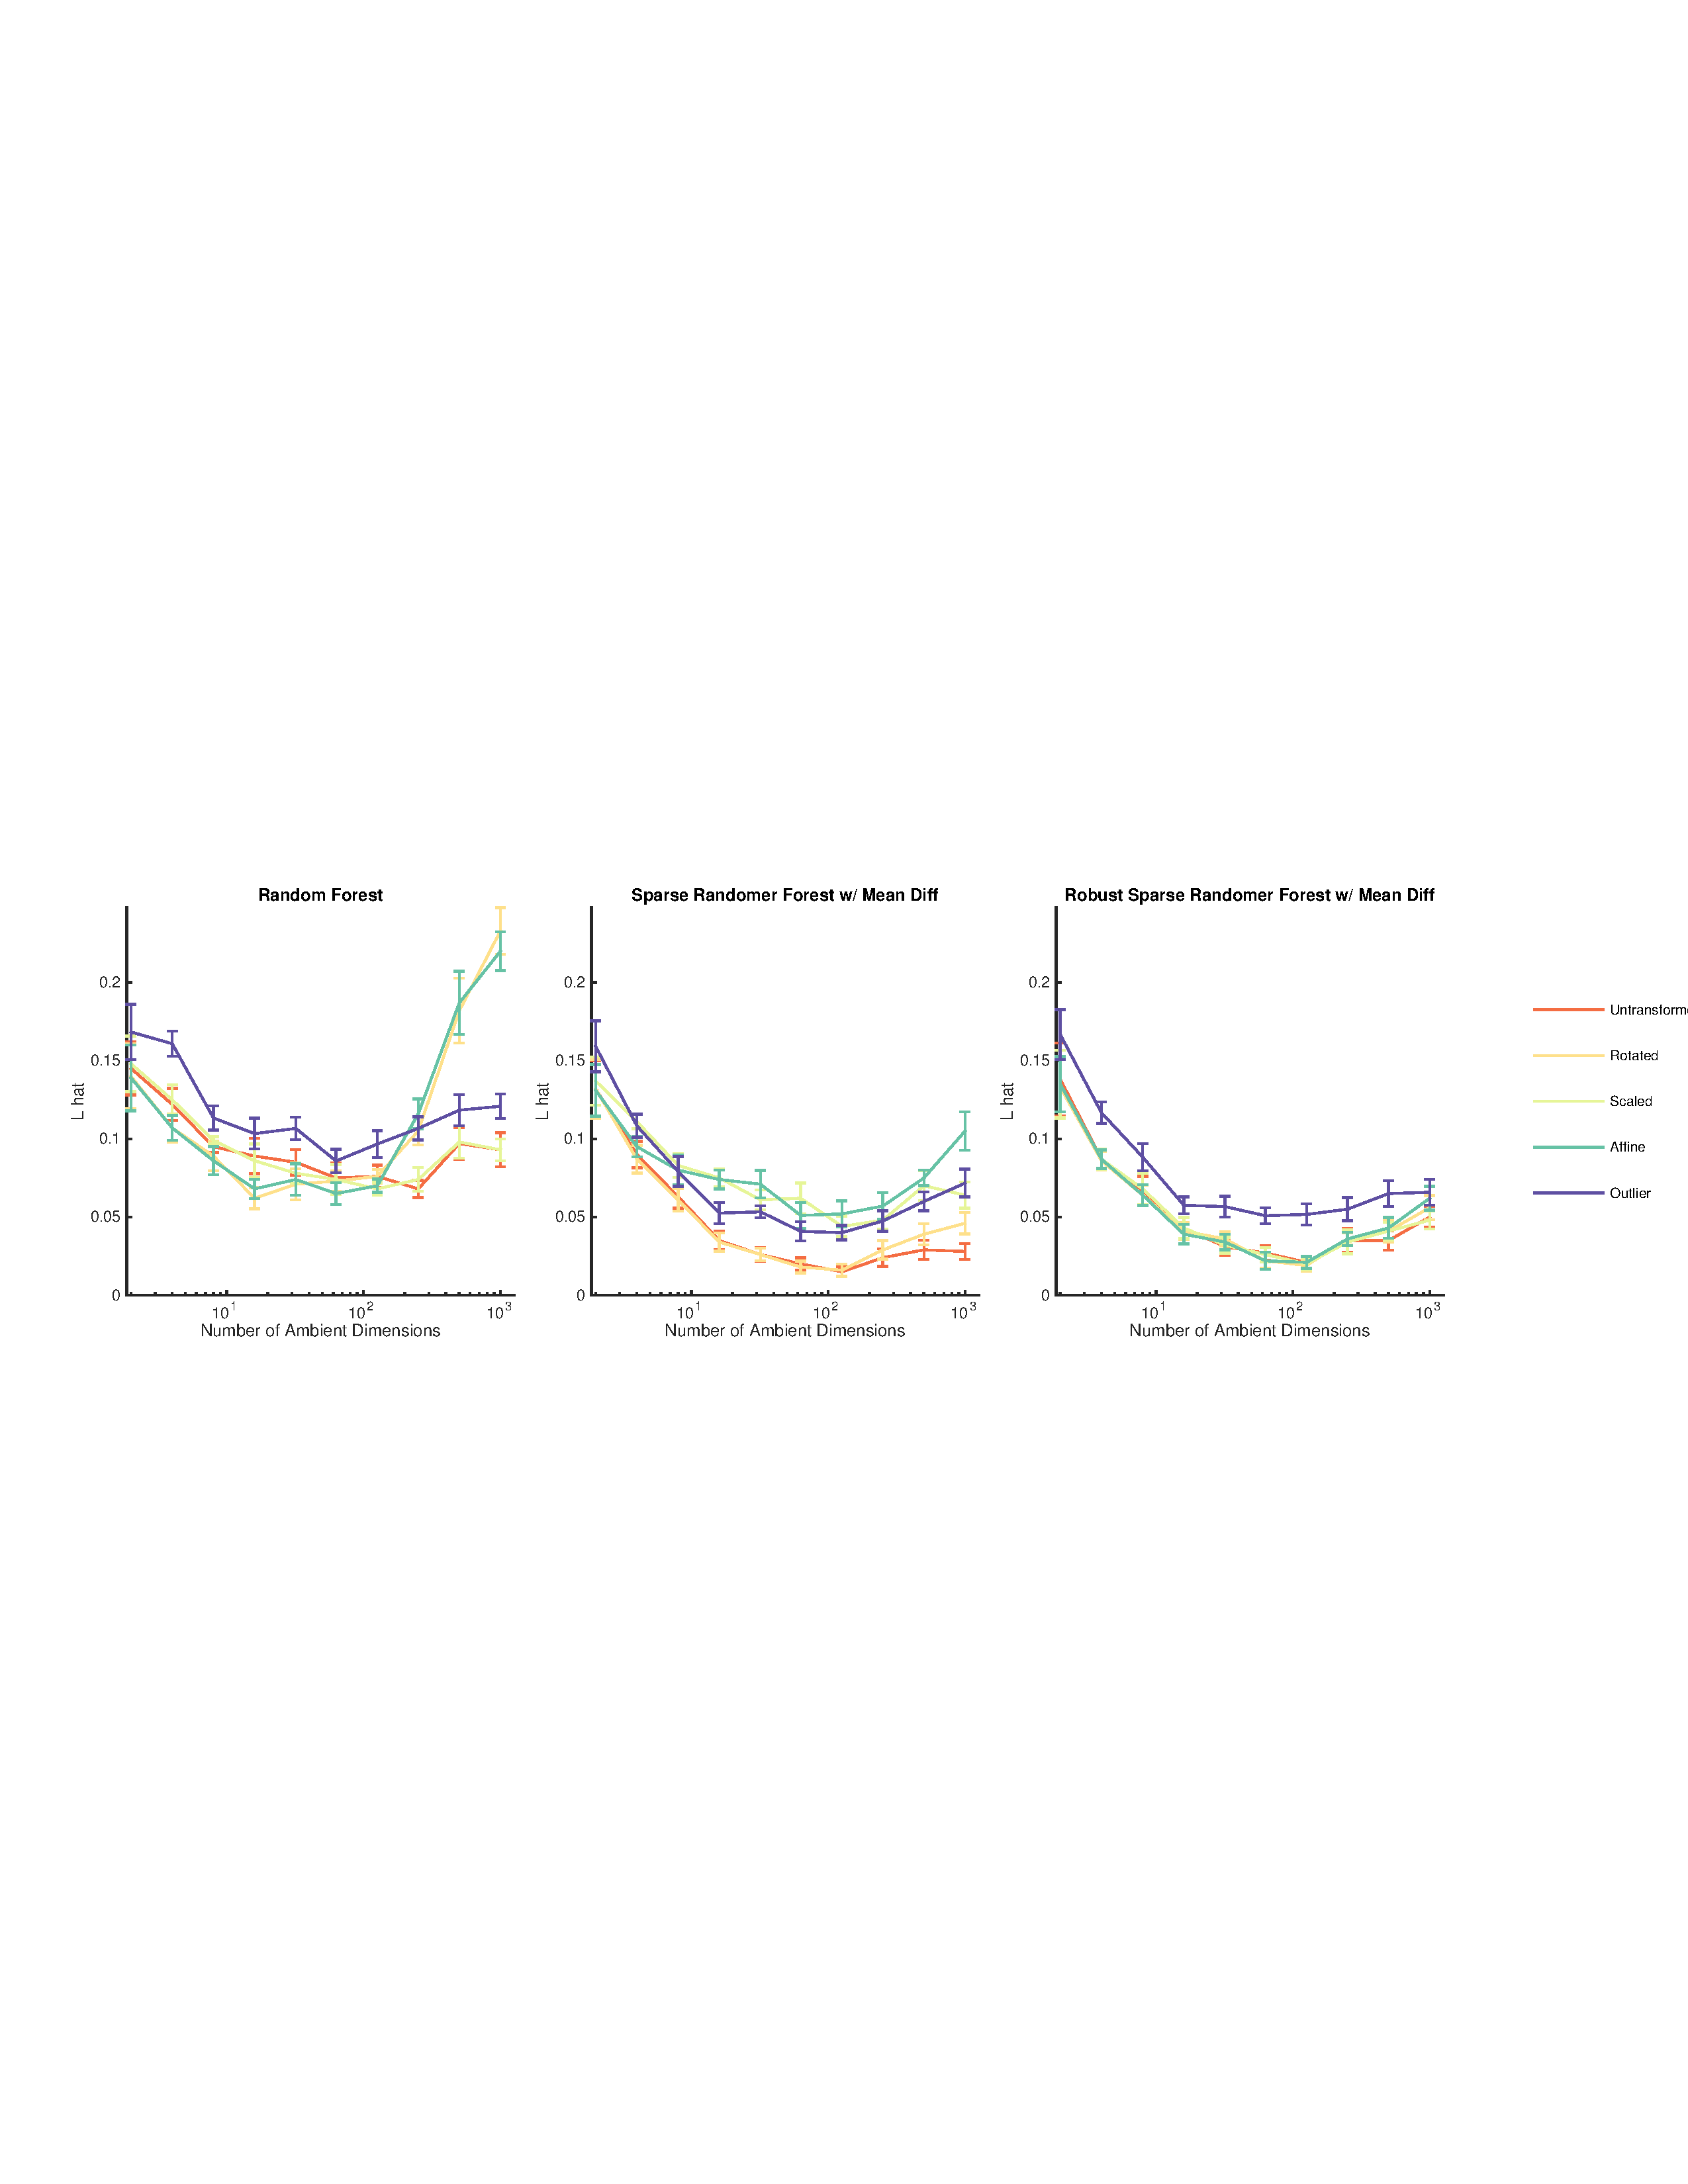
\includegraphics[trim=0in 0.9in 0in .09in, clip=true, width=\linewidth]{Fig3_Invariance_v2}
\end{center}
\caption{The effect of various transformations applied to the Trunk simulation (see Methods for details) on classification performance of (A) Random Forest, (B) Randomer Forest (sparse+delta) and (C) Randomer Forest (sparse+delta+robust). Except for scaling, classification performance of RF is compromised by all transformations. R'er F (s+d) is invariant to rotation, and R'er F (s+d+r) is invariant to rotation, scaling, and affine transformations.}
\end{figure}

\begin{figure}[h]
\begin{center}
%\framebox[4.0in]{$\;$}
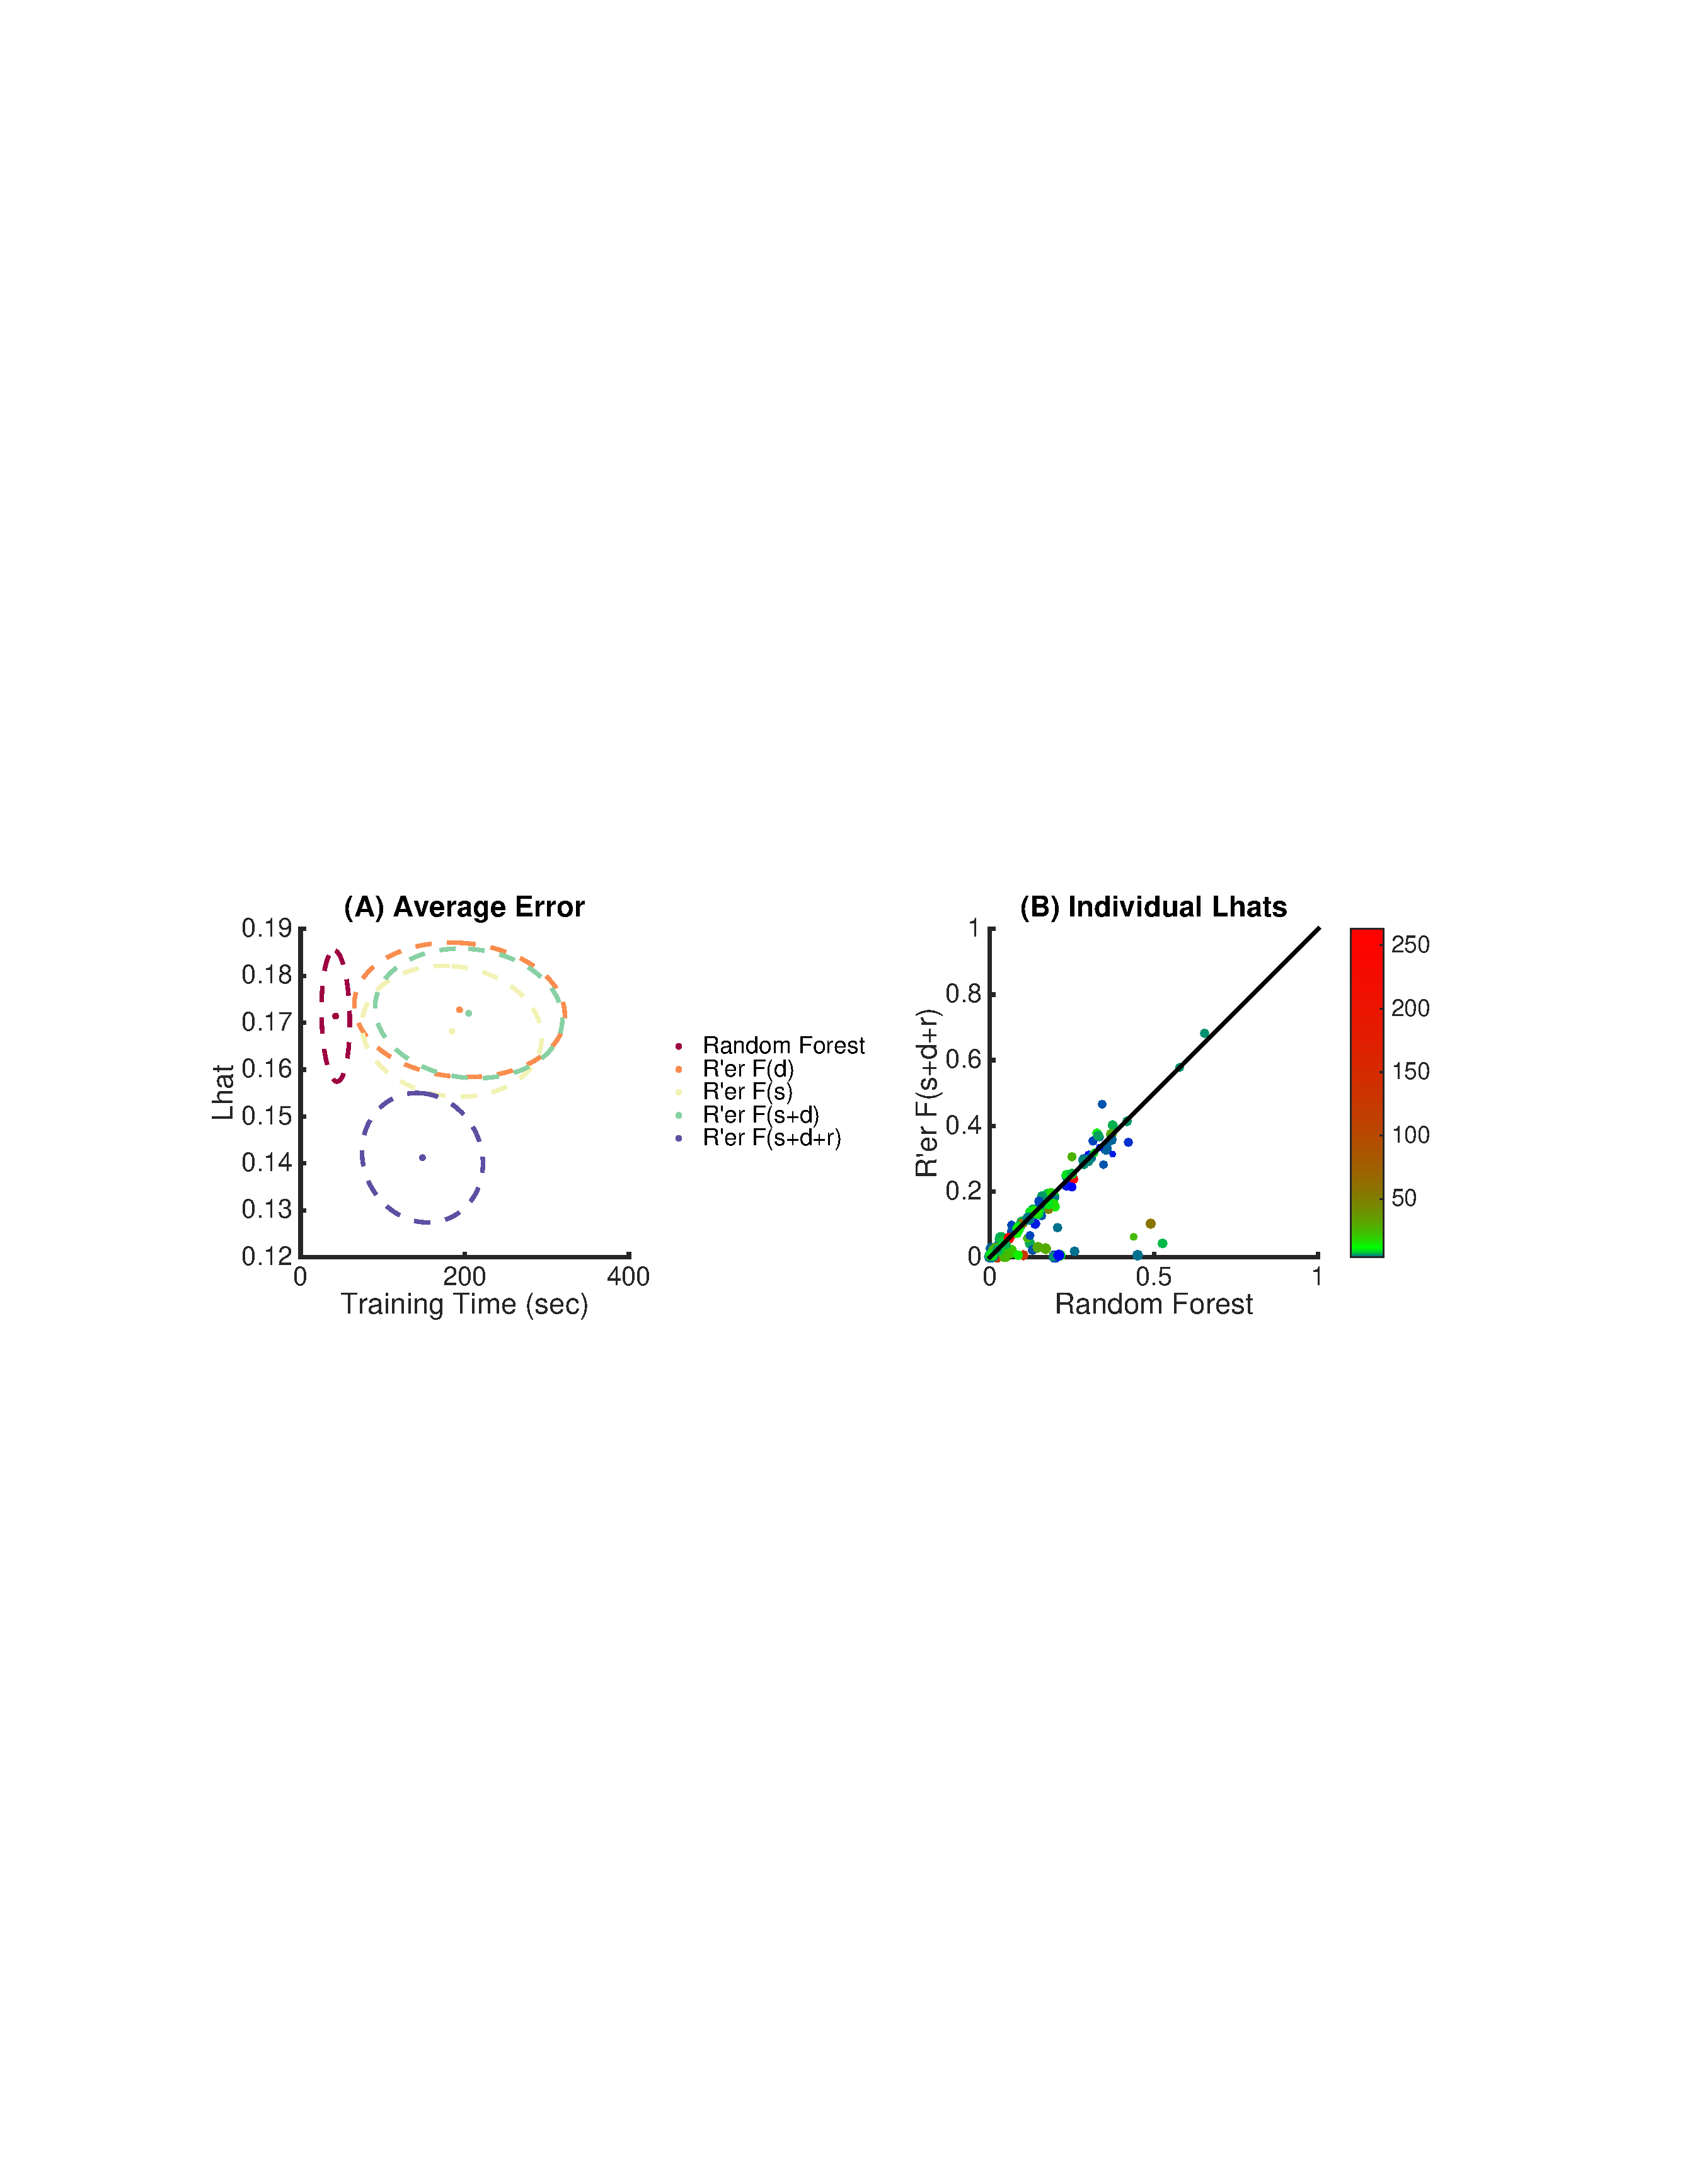
\includegraphics[trim=0in 2.3in 0in 2.3in, clip=true, width=\linewidth]{Fig4}
\end{center}
\caption{(A) Classification error and training time of Random Forest and Randomer Forests averaged over 121 real datasets. Dashed lines represent a 0.1 SD level curve. (B) Classification error of Randomer Forest (sparse+delta+robust) vs. that of Random Forest for each of the 121 datasets. The black line indicates equal classification error of the two algorithms. Color indicates dimensionality of the datasets and size of points indicates number of samples.}
\end{figure}

\end{document}